% ============================================================
% MLOps for Football World Cup Prediction — condensed paper
% IEEE Conference Format — IEEEtran (~7 pages)
% Compile: pdflatex -> bibtex -> pdflatex -> pdflatex
% ============================================================

\documentclass[conference]{IEEEtran}

\usepackage[T1]{fontenc}
\usepackage[utf8]{inputenc}
\usepackage{cite}
\usepackage{amsmath,amssymb}
\usepackage{graphicx}
\usepackage{booktabs}
\usepackage{hyperref}
\usepackage{tikz}
\usetikzlibrary{positioning,arrows.meta}
\usepackage{pgfgantt}

% Include figure only if present (optional assets from full report)
\newcommand{\maybegraphic}[2]{%
  \IfFileExists{#1}{%
    \includegraphics[width=#2]{#1}%
  }{%
    \fbox{\parbox{0.9\linewidth}{\centering\small\textit{Figure file not found:} \texttt{#1}}}%
  }%
}

\begin{document}

\title{MLOps for Football World Cup Prediction:\\
A Multi-Model Comparison with Structured Model Promotion}

\author{
  \IEEEauthorblockN{Tom Farnschläder}
  \IEEEauthorblockA{\textit{Tampere University}\\
  Tampere, Finland\\
  tom.farnschlaeder@tuni.fi}
  \and
  \IEEEauthorblockN{Sergio Moreschini}
  \IEEEauthorblockA{\textit{Tampere University}\\
  Tampere, Finland\\
  sergio.moreschini@tuni.fi}
}

\maketitle

\begin{abstract}
Predicting football World Cup outcomes is challenging because national-team
data are sparse and irregular, and low-scoring matches are inherently noisy.
We present a structured MLOps pipeline that automates ingestion from two
external sources through Bronze/Silver/Gold feature engineering to Monte Carlo
simulation of the 2026 FIFA World Cup.
Nine candidate models spanning statistical, Bayesian, time-series, classical
machine learning, and deep-learning families are compared under explicit
hypotheses, with experiments tracked in MLflow and data versioned with DVC.
Models pass through a three-environment lifecycle (Experimental, QA, Deploy)
with walk-forward tuning on Poisson negative log-likelihood and holdout
selection on Ranked Probability Score against the 2022 World Cup.
Permutation importance shows that Elo differential dominates all families;
Ridge is promoted as production champion despite ranking seventh in
cross-validation.
We discuss threats to validity for sparse national-team data and the expanded
2026 tournament format.
\end{abstract}

\begin{IEEEkeywords}
MLOps, football prediction, machine learning pipelines, model lifecycle
\end{IEEEkeywords}

% ============================================================
\section{Introduction}
\label{sec:intro}

Predicting football match outcomes has attracted substantial interest since
Maher~\cite{maher1982modelling} showed that scores can be modelled as Poisson
processes conditioned on team attack and defence strength.
Club football benefits from dense weekly fixtures; national teams play only a
few international windows per year, squads rotate, and competitive stakes vary
from friendlies to World Cup finals.

In parallel, MLOps~\cite{google_mlops,moreschini2022mlops} brings software-engineering
discipline to ML systems: versioned data, tracked experiments, explicit
promotion gates, and automated retraining.
This work applies that discipline to World Cup prediction rather than treating
modelling as a one-off notebook exercise.

We make two contributions:
\begin{itemize}
  \item \textbf{Pipeline design:} a local-first MLOps pipeline with
  Bronze/Silver/Gold data layers, a three-environment model lifecycle
  (Experimental~$\to$~QA~$\to$~Deploy), DVC-versioned artifacts, and
  MLflow-tracked runs.
  \item \textbf{Multi-model comparison:} nine models across five families,
  evaluated under four stated hypotheses with permutation-based feature
  importance.
\end{itemize}

Figure~\ref{fig:architecture} summarises the end-to-end flow from ingestion
through model promotion to tournament simulation.
Section~\ref{sec:background} reviews MLOps and football score modelling.
Section~\ref{sec:related} positions related work.
Section~\ref{sec:developing} states general pipeline design decisions;
Section~\ref{sec:architecture} records our architectural choices.
Section~\ref{sec:implementation} describes implementation and results.
Sections~\ref{sec:discussion} and~\ref{sec:conclusion} discuss findings and conclude.

\begin{figure}[t]
  \centering
  \maybegraphic{../figures/Architecture_final.png}{0.95\columnwidth}
  \caption{End-to-end MLOps pipeline: Bronze/Silver/Gold data path,
  three model environments, and Monte Carlo tournament simulation.}
  \label{fig:architecture}
\end{figure}

% ============================================================
\section{Background}
\label{sec:background}

MLOps extends the DevOps loop with ML-specific activities (data exploration,
feature engineering, model validation, and experiment optimisation) while
retaining continuous integration and delivery~\cite{moreschini2022mlops}.
A practice unique to ML systems is \emph{continuous training} (CT): automated
retraining as new data arrives~\cite{ossara2023}.
Google's maturity model~\cite{google_mlops} distinguishes three automation
levels: Level~0 (manual steps), Level~1 (automated training pipeline with
reusable components), and Level~2 (full CI/CD of pipeline code and deployment).
Industry practice often decomposes MLOps as
$\text{MLOps} = \text{DevOps} + \text{DataOps} + \text{ModelOps}$~\cite{databricks_bigbook}:
DevOps covers code and release engineering; DataOps covers reproducible data
management; ModelOps covers experiment tracking, registry, and promotion.

Figure~\ref{fig:mlops_decomp} sketches the three operational domains and their
typical tooling layers.
Our project-specific mapping of tools to these domains appears in
Section~\ref{sec:architecture}.

\begin{figure}[t]
  \centering
  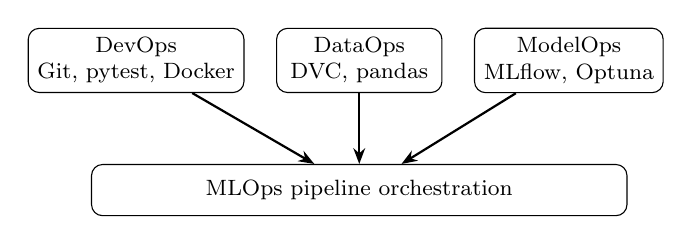
\begin{tikzpicture}[
    node distance=0.55cm and 0.4cm,
    box/.style={draw, rounded corners, align=center, font=\footnotesize,
                minimum width=2.1cm, minimum height=0.65cm},
    arr/.style={-{Stealth[length=2mm]}, thick}
  ]
    \node[box] (dev) {DevOps\\Git, pytest, Docker};
    \node[box, right=of dev] (data) {DataOps\\DVC, pandas};
    \node[box, right=of data] (model) {ModelOps\\MLflow, Optuna};
    \node[box, below=0.9cm of data, minimum width=6.8cm] (mlops)
      {MLOps pipeline orchestration};
    \draw[arr] (dev) -- (mlops);
    \draw[arr] (data) -- (mlops);
    \draw[arr] (model) -- (mlops);
  \end{tikzpicture}
  \caption{MLOps as DevOps + DataOps + ModelOps (conceptual).}
  \label{fig:mlops_decomp}
\end{figure}

For football scores, Maher~\cite{maher1982modelling} modelled each side's goals
as independent Poisson processes with attack, defence, and home-advantage
parameters.
Dixon and Coles~\cite{dixon1997modelling} added time decay and a low-score
correction for negative correlation between home and away goals.
Karlis and Ntzoufras~\cite{karlis2003analysis} decomposed a match into three
Poisson components (home-specific $\lambda_1$, away-specific $\lambda_2$, and
shared $\lambda_3$) to induce dependence between scorelines.
Negative Binomial and Bayesian extensions relax equidispersion and yield full
predictive distributions respectively.

National-team strength is often summarised by Elo ratings~\cite{eloratings},
which update after each match from result and expected-score differential with
tournament-weighted $K$-factors.
Elo provides a continuous cross-confederation quality measure without squad-level
data, which is a practical abstraction for sparse international calendars.

% ============================================================
\section{Related Works}
\label{sec:related}

Moreschini et al.~\cite{moreschini2022mlops} survey MLOps from DevOps evolution,
automation maturity, and tooling perspectives.
Their OSSARA pipeline~\cite{ossara2023} demonstrates a complete Level-1 style
workflow for open-source software abandonment risk assessment: DVC for data, 
MLflow for experiments, explicit staging environments, and scheduled 
retraining. 
We apply the same pipeline engineering pattern to national-team football analytics.

Groll et al.~\cite{groll2019prediction} predict major tournaments with
team-specific regularised Poisson regression on historical results; their focus
is statistical modelling rather than operational ML lifecycle.
We adopt Poisson-family candidates and tournament simulation but embed them in
a reproducible MLOps pipeline with nine heterogeneous model families and
explicit promotion logic.


% ============================================================
\section{Developing an MLOps Pipeline}
\label{sec:developing}

Building an MLOps pipeline requires decisions that precede any single model
choice~\cite{google_mlops,databricks_bigbook}.

\textbf{Data versioning.}
Raw snapshots, transformed tables, and model artifacts must be reproducible 
and separable from code. A dedicated versioning tool (e.g.\ DVC) tracks each 
pipeline stage's inputs and outputs so any state can be exactly reproduced.

\textbf{Experiment tracking.}
Every training run should log parameters, metrics, and artifacts so that
promotion decisions are auditable.
A central experiment store (e.g.\ MLflow) supports comparison across model
families and pipeline stages.

\textbf{Promotion logic.}
Experimentation, validation, and production must be separated by explicit gates.
Tuning metrics need not equal deployment metrics: goal-rate likelihood may tune
hyperparameters while outcome-level scores select champions for simulation.

\textbf{Deployment model.}
Model-based deployment promotes frozen artifacts; code-based deployment promotes
the training pipeline and retrains in each environment on progressively larger
data~\cite{databricks_bigbook}.
The latter supports automated retraining without manual artifact handoff.

\textbf{Automation scope.}
Level-1 automation (scheduled data refresh and retrain) is often sufficient for
event-driven systems such as a single tournament; full CI/CD of pipeline code
(Level~2) can follow once the core loop is stable.

% ============================================================
\section{System Architecture}
\label{sec:architecture}

\subsection{Architectural choices}

We target Google MLOps \textbf{Level~1}~\cite{google_mlops}: DVC orchestrates
Bronze$\to$Silver$\to$Gold rebuilds; a common Python interface trains all
candidates; MLflow logs every run; a scheduled trigger handles retraining and
inference.
Full CI/CD of pipeline code (Level~2) is deferred.

Following the DataOps/ModelOps split~\cite{databricks_bigbook,ossara2023},
\textbf{DVC} versions raw snapshots, Silver Parquet, and Gold artifacts;
\textbf{MLflow} tracks experiments and manages registry promotion;
\textbf{Git} and \textbf{pytest} provide the DevOps base.
DagsHub is used as a unified remote for data, code and model artifacts.

We adopt \textbf{code-based deployment}~\cite{databricks_bigbook}: the three
environments share identical training code; what advances is a validated
configuration, not a frozen artifact.
Experimental trains on pre-2022 Gold; QA evaluates on the 2022 World Cup holdout;
Deploy refits the champion on all available Gold at run time.

\subsection{Data and model lifecycle}

\textbf{Bronze} stores immutable API-Football JSON and Elo TSV snapshots.
\textbf{Silver} is schema-validated, season-partitioned Parquet, joining data 
from both sources and adding context, such as competition tiers or knockout 
flags.
\textbf{Gold} is one row per match with strictly time-aware features (rolling
form, Elo composites, context flags); no future information enters any column.

Model development uses three environments backed by MLflow registry models
(Figure~\ref{fig:architecture}):
\begin{enumerate}
  \item \textbf{Experimental:} all nine candidates are tuned by Optuna on 
  walk-forward CV Poisson Negative Log-Likelihood (NLL). The best-performing configuration for each
  model advances to QA.
  \item \textbf{QA:} the nine model configurations are backtested on all 64 
  WC~2022 matches. The artifacts of the model with the lowest holdout Ranked 
  Probability Score (RPS) is registered as challenger for audit.
  \item \textbf{Deploy:} the challenger is compared against the existing champion model. The one with the lower RPS is registered as champion, refitted on the full Gold data and used for inference. The other eight model configurations from QA are refitted in parallel for live monitoring.
\end{enumerate}

\subsection{Tool stack}

\begin{table}[h]
  \caption{Selected tool stack}
  \label{tab:tools}
  \begin{tabular}{@{}ll@{}}
    \toprule
    Purpose & Tool \\
    \midrule
    Data pipeline & Python, pandas, numpy \\
    Statistical / TS models & statsmodels, PyMC \\
    ML / DL & scikit-learn, XGBoost, Keras \\
    Tuning \& tracking & Optuna, MLflow \\
    Versioning & DVC, Git \\
    Ops & pytest, Docker, Cloud Run Jobs \\
    \bottomrule
  \end{tabular}
\end{table}

% ============================================================
\section{Implementing the Pipeline}
\label{sec:implementation}

This section maps the architecture to the concrete implementation: dual-source
ingestion, nine model candidates spanning five model families, explicit 
promotion, cloud scheduling, and live monitoring.

\subsection{Data pipeline (DataOps)}
\label{sec:impl_data}

\textbf{Sources.}
To cover both ELO scores and in-game statistics, two data sources were used. 
API-Football supplies national-team fixtures and per-match statistics.
Elo ratings (eloratings.net) supply self-regulatory strength estimates as
per-team TSV histories.
All national team data from 2018 onwards was used.

\textbf{Bronze--Silver.}
The raw JSON and TSV are DVC-tracked.
Silver retains finished matches only (\texttt{FT}/\texttt{AET}/\texttt{PEN}),
joins statistics by \texttt{fixture\_id} and encodes a
\texttt{stats\_tier} (\texttt{full}/\texttt{partial}/\texttt{cards\_only}/\texttt{none}),
resolves team identity via a curated mapping, filters youth and non-FIFA
entities, assigns competition tier (1=World Cup finals through 4=friendlies)
and a \texttt{is\_knockout} flag, joins pre-match Elo by
\texttt{merge\_asof}, and derives \texttt{is\_neutral}.
Schema validation runs before Parquet write.
Table~\ref{tab:silver_schema} summarises the resulting 72-column schema.

\begin{table}[h]
  \caption{Silver column groups (72 total)}
  \label{tab:silver_schema}
  \begin{tabular}{@{}lc@{}}
    \toprule
    Group & Count \\
    \midrule
    Match identity & 14 \\
    Teams (ID, name, ISO, conf.) & 10 \\
    Goals (final, HT, FT, ET, pen.) & 10 \\
    Elo (pre/post, both sides) & 4 \\
    Match statistics (16 per side) & 32 \\
    Quality flags & 2 \\
    \midrule
  \textbf{Total} & \textbf{72} \\
    \bottomrule
  \end{tabular}
\end{table}

\textbf{Gold.}
Rolling means of goals for/against (10 prior matches), rolling tactical profiles
from matches with statistics coverage, Elo difference and sum, days since last match 
as a squad-cohesion proxy (tactical familiarity, coordination, time-as-a-unit), and 
context flags on tournament and match level are
computed with strict temporal ordering to make sure each feature uses only
prior matches and avoid data leakage.
Rolling tactical columns use volume (\texttt{total\_shots}) and precision
(\texttt{shot\_precision}) rather than linearly dependent shot subtypes;
opponent-suffered stats were excluded to avoid confounding style with opponent
quality.
K-means clustering on five rolling tactical dimensions yielded silhouette scores
below 0.40 for all $k\in\{2,\ldots,10\}$
(Figure~\ref{fig:cluster_k}); raw continuous columns were retained instead.

\begin{figure}[h]
  \centering
  \maybegraphic{../figures/cluster_experiment_v2.png}{0.95\columnwidth}
  \caption{Elbow and silhouette analysis for tactical clustering (not used in Gold).}
  \label{fig:cluster_k}
\end{figure}

WC~2026 co-hosts (USA, Canada, Mexico) receive \texttt{is\_neutral=False} at
home venues in the group stage via a deterministic Gold override; knockout
overrides use venue-to-country mapping in the tournament JSON during
simulation.

\subsection{Model lifecycle (ModelOps)}
\label{sec:impl_model}

The prediction target is the joint distribution over $(home\_goals, away\_goals)$.

Match outcomes are derived by marginalising the predicted score distribution: 
$P(\text{home win}) = \sum_{i>j} P(H{=}i, A{=}j)$, where home and away goals 
are treated as (conditionally) independent Poisson variates with rates 
$\hat{\lambda}_h$ and $\hat{\lambda}_a$. Tournament advancement probabilities 
are then obtained by Monte Carlo simulation ($n_\mathrm{sims}=10{,}000$ 
paths), sampling scorelines for all $\binom{48}{2} = 1{,}128$ 
possible matchups and propagating uncertainty through the full knockout tree.


Table~\ref{tab:models} lists nine candidates spanning five families.
Hyperparameters are tuned with Optuna (50 TPE trials, walk-forward CV).
\textbf{Tuning} minimises Poisson NLL; \textbf{QA gating} uses holdout RPS.
The two metrics are deliberately decoupled.

\textbf{Poisson NLL} rewards placing probability mass near the actual
scoreline:
\begin{equation}
  \text{NLL} = -\frac{1}{N}\sum_{i=1}^{N}
  \bigl[\log P(h_i \mid \hat{\lambda}_{h,i})
       + \log P(a_i \mid \hat{\lambda}_{a,i})\bigr]
\end{equation}
where $h_i, a_i$ are observed goals and $\hat{\lambda}_{h,i},
\hat{\lambda}_{a,i}$ the predicted Poisson rates.
NLL is agnostic to outcome ordering, making it a stable signal for
hyperparameter search.

\textbf{Ranked Probability Score} evaluates the cumulative W/D/L distribution:
\begin{equation}
  \text{RPS} = \frac{1}{K{-}1} \sum_{k=1}^{K-1}
  \Bigl( \sum_{i=1}^{k} p_i - \sum_{i=1}^{k} o_i \Bigr)^{\!2}
\end{equation}
where $p_i$ is the predicted probability and $o_i \in \{0,1\}$ the observed
indicator for outcome $i$, with outcomes ordered away win, draw, home win
($K{=}3$).
RPS directly measures what matters for tournament advancement prediction.
Using RPS as the tuning objective would create a draw-hedging incentive,
since draw occupies the middle ordinal position and a confident incorrect
draw prediction never incurs the maximum penalty.

All nine candidates advance to QA after an initial top-4 gate proved
misleading when CV and holdout rankings diverged
(Section~\ref{sec:impl_results}).


\begin{table}[h]
  \caption{Candidate models}
  \label{tab:models}
  \begin{tabular}{@{}cll@{}}
    \toprule
    \# & Model & Family \\
    \midrule
    1 & Poisson GLM & Statistical \\
    2 & Negative Binomial GLM & Statistical \\
    3 & Bayesian Poisson & Bayesian \\
    4 & SARIMAX & Time-series \\
    5 & Ridge & ML baseline \\
    6 & Random Forest & ML ensemble \\
    7 & XGBoost & Boosting \\
    8 & LSTM & Deep learning \\
    9 & 1D CNN & Deep learning \\
    \bottomrule
  \end{tabular}
\end{table}

\textbf{Per-model design notes.}
The \textbf{Poisson GLM} implements the Karlis--Ntzoufras bivariate
Poisson~\cite{karlis2003analysis}: a match is decomposed into three Poisson
components ($\lambda_1$, $\lambda_2$, shared $\lambda_3$), with $\lambda_3$
inducing score dependence across both scorelines.
This was chosen over Dixon--Coles~\cite{dixon1997modelling} because Elo
ratings and 10-match rolling form already impose recency weighting on the
feature side, making explicit likelihood-level time decay largely redundant.
The \textbf{NegBin GLM} fits independent home/away marginals rather than a
bivariate model: the Poisson additivity that underpins the
Karlis--Ntzoufras construction does not extend to Negative Binomial variates
under differing dispersion.
\textbf{Bayesian Poisson} uses PyMC's NUTS sampler to produce full posterior
predictive distributions.
A Bayesian bivariate variant was implemented but excluded: the custom
log-PMF required PyMC to auto-differentiate through complex tensor
operations at every NUTS leapfrog step, making each MCMC step
${\sim}50\times$ slower with no CV NLL improvement.
\textbf{SARIMAX} uses an integer match-index time axis rather than calendar
dates, treating multi-month gaps identically to within-window spacing---an
acknowledged limitation (Section~\ref{sec:threats}).

\textbf{Hypotheses.}
\begin{description}
  \item[H1] \texttt{elo\_diff} is the dominant feature across families. Elo 
  ratings encode cumulative match history into a single continuous quality signal 
  without requiring squad-level data, making them the most information-dense 
  feature available for national teams.
  \item[H2] Poisson GLM is a competitive baseline despite simpler structure. 
  Football goal counts are well-approximated by Poisson 
  processes~\cite{maher1982modelling},
  so a correctly specified GLM is expected to capture the core signal that more
  complex architectures must also learn.
  \item[H3] Deep learning underperforms relative to complexity given sparse data. 
  LSTM and CNN require long per-team sequences to generalise; national teams play
  only around 10 matches per year, leaving too few observations to train deep
  architectures without overfitting.
  \item[H4] Bayesian Poisson yields best-calibrated goal predictions. Full 
  MCMC posterior predictive distributions propagate parameter uncertainty
  into score predictions, which should translate into better-calibrated goal 
  distributions than point-estimate models.
\end{description}

\subsection{Training and deployment}
\label{sec:impl_deploy}

Training uses 3{,}903 pre-WC~2022 matches; the QA holdout is 64 WC-tier
matches from Qatar 2022 (\texttt{competition\_tier=1}).

\textbf{Champion selection.}
The QA candidate with the lowest holdout RPS is designated the challenger.
If no current champion exists, the challenger is promoted unconditionally;
otherwise, promotion requires a strict RPS improvement over the incumbent.
On successful promotion, the champion is refit on all available Gold
(2018 through the latest ingested match) using the hyperparameters selected
during the experimental phase.
This production-refit artifact is registered as \texttt{wc\_production} in
the MLflow model registry and promoted via the \texttt{champion} alias.

\textbf{Subsequent automated refits.}
Once the initial selection is complete, subsequent trigger cycles that
exceed the retraining threshold bypass the candidate tournament entirely.
The trigger loads the champion's model class and hyperparameters from the
registry and refits on the latest full Gold.
The original QA holdout metrics are forwarded unchanged to the new MLflow
run, preserving audit continuity.
This separation of \emph{model selection} (fixed at QA) from
\emph{model refresh} (automated on new data) avoids a redundant multi-hour
candidate tournament on every data update.

\textbf{Shadow models.}
Eight non-champion candidates are refit on the same full Gold window using
each candidate's Optuna-tuned hyperparameters.
These shadow refits feed the WC~2026 monitoring leaderboard so all nine models
can be compared on a like-for-like basis without confounding model family with
data recency.
No re-tuning occurs; model selection is frozen.

\textbf{Ingestion trigger and continuous training.}
Freshness checks use (1)~Elo SHA-256 digest change and (2)~API-Football
incremental window with all fixtures settled.
An OR gate triggers \texttt{dvc repro} when either source updates.
The initial run executes the full
Experimental$\to$QA$\to$Deploy pipeline; subsequent runs refit the champion
only when Gold grows by $\geq$10 rows, forwarding original QA metrics for
audit continuity.
Tournament \texttt{inference\_only} mode rebuilds Gold rolling features from
settled WC matches without retraining.
Figure~\ref{fig:ct_architecture} illustrates the trigger, training, and
inference paths.

\begin{figure}[h]
  \centering
  \maybegraphic{../figures/architecture_ct_pipeline.png}{0.95\columnwidth}
  \caption{Trigger, continuous training, and inference paths.}
  \label{fig:ct_architecture}
\end{figure}

\textbf{Cloud deployment.}
The pipeline is packaged in Docker on Cloud Run Jobs with dual Cloud
Scheduler entries.
Daily runs capture the last friendly matches of qualified teams before the
tournament starts; 30-minute runs during the World Cup keep predictions
up-to-date with a frozen champion (\texttt{inference\_only} mode).

\textbf{Live monitoring.}
Every 30-minute inference cycle predicts all $1{,}128$ pairings with all
nine models (champion plus eight shadow versions) and logs long-format
results as MLflow artifacts.
After each settled WC~2026 match, a monitoring step joins the actual
scoreline with the most recent inference whose timestamp is \emph{strictly
earlier} than kickoff. The strict inequality is essential because a later
inference cycle already incorporates the result into Gold features, so
using it would leak post-match information into the evaluation.
Per-match RPS, Poisson NLL, RMSE\textsubscript{home}, and
RMSE\textsubscript{away} are computed for each of the nine models from
predicted Poisson rates.
For each model, a rolling-mean RPS over the last 24 scored matches
(one group-stage matchday: 12~groups $\times$ 2~matches) is compared
against $1.3\times$ that model's WC~2022 holdout RPS baseline; a breach
emits a warning captured by Cloud Logging.
Models with fewer than 24 scored matches (the first group matchday) are 
skipped to suppress early-tournament noise.
No automated promotion occurs under any alert condition: mid-tournament
retraining is out of scope because ${\sim}$5~weeks of WC matches is too
short for statistically meaningful drift detection.

\subsection{Results}
\label{sec:impl_results}

Table~\ref{tab:qa_results} reports WC~2022 holdout metrics.
Ridge wins on RPS (0.2250) despite ranking seventh in CV NLL (2.8471); the
CV NLL leader (NegBin GLM, 2.7576) drops to seventh on holdout RPS (0.2294).
Excluding CNN, the remaining eight models lie within a 0.0046 RPS band
(0.2250--0.2296), making them statistically indistinguishable on 64~matches.

Outcome accuracy tells a complementary story: LSTM leads at 54.7\% (35/64)
while Ridge achieves only 50.0\% (32/64).
For the downstream Monte Carlo simulation, which consumes full probability
distributions, RPS is the appropriate selection metric; Ridge was promoted.
The CV--holdout ranking reversal is analysed in
Section~\ref{sec:discussion}.

\begin{table}[h]
  \caption{QA holdout (64 WC~2022 matches, sorted by holdout RPS).
  CV NLL is the walk-forward tuning metric; holdout RPS is the gating
  metric.}
  \label{tab:qa_results}
  \begin{tabular}{@{}lcccc@{}}
    \toprule
    Model & CV NLL & RPS & NLL & Acc. \\
    \midrule
    Ridge            & 2.847 & \textbf{0.2250} & 3.023 & 50.0\% \\
    Random Forest    & 2.768 & 0.2255 & 3.012 & 53.1\% \\
    XGBoost          & 2.767 & 0.2263 & 3.011 & 51.6\% \\
    Poisson GLM      & 2.763 & 0.2284 & 3.030 & 53.1\% \\
    LSTM             & 2.821 & 0.2289 & 3.099 & 54.7\% \\
    Bayesian Poisson & 2.759 & 0.2289 & 3.038 & 51.6\% \\
    NegBin GLM       & 2.758 & 0.2294 & 3.041 & 53.1\% \\
    SARIMAX          & 3.016 & 0.2336 & 3.315 & 50.0\% \\
    1D CNN           & 3.039 & 0.2479 & 3.166 & 42.2\% \\
    \bottomrule
  \end{tabular}
\end{table}

Table~\ref{tab:importance} reports permutation importance measured as holdout
RPS degradation.
Elo difference ranks first in all nine models with degradation scores
10--100$\times$ larger than any secondary feature.
Deep-learning models assign relatively more weight to home advantage, likely
compensating for weaker Elo exploitation.

\begin{table*}[t]
  \caption{Top-3 permutation importance (RPS degradation)}
  \label{tab:importance}
  \small
  \begin{tabular}{@{}lccc@{}}
    \toprule
    Model & \#1 & \#2 & \#3 \\
    \midrule
    Random Forest & \texttt{elo\_diff} \scriptsize{+.121}
      & \texttt{elo\_sum} \scriptsize{+.002}
      & \texttt{roll\_goals\_ag$_h$} \scriptsize{+.002} \\
    SARIMAX & \texttt{elo\_diff} \scriptsize{+.110}
      & \texttt{roll\_goals\_ag$_h$} \scriptsize{+.002}
      & \texttt{elo\_sum} \scriptsize{+.000} \\
    NegBin GLM & \texttt{elo\_diff} \scriptsize{+.104}
      & \texttt{roll\_goals\_ag$_h$} \scriptsize{+.001}
      & \texttt{comp\_tier} \scriptsize{+.001} \\
    Bayesian Poisson & \texttt{elo\_diff} \scriptsize{+.103}
      & \texttt{rest\_diff} \scriptsize{+.001}
      & \texttt{roll\_goals\_ag$_h$} \scriptsize{+.001} \\
    Poisson GLM & \texttt{elo\_diff} \scriptsize{+.102}
      & \texttt{roll\_goals\_ag$_h$} \scriptsize{+.001}
      & \texttt{comp\_tier} \scriptsize{+.001} \\
    XGBoost & \texttt{elo\_diff} \scriptsize{+.098}
      & \texttt{roll\_tac\_poss$_a$} \scriptsize{+.002}
      & \texttt{roll\_goals\_ag$_h$} \scriptsize{+.002} \\
    LSTM & \texttt{elo\_diff} \scriptsize{+.095}
      & \texttt{is\_neutral} \scriptsize{+.005}
      & \texttt{comp\_tier} \scriptsize{+.002} \\
    Ridge & \texttt{elo\_diff} \scriptsize{+.062}
      & \texttt{roll\_goals\_ag$_h$} \scriptsize{+.004}
      & \texttt{roll\_goals\_ag$_a$} \scriptsize{+.002} \\
    1D CNN & \texttt{elo\_diff} \scriptsize{+.055}
      & \texttt{is\_neutral} \scriptsize{+.005}
      & \texttt{comp\_tier} \scriptsize{+.004} \\
    \bottomrule
  \end{tabular}
\end{table*}

% ============================================================
\section{Discussion}
\label{sec:discussion}

\subsection{General}

\textbf{H1 (confirmed):} \texttt{elo\_diff} ranks first in every family;
secondary features contribute at most marginal corrections.

\textbf{H2 (confirmed):} The bivariate Poisson GLM is fourth on holdout RPS and 
competitive on CV NLL. It is a strong baseline that complex models do not clearly 
beat once Elo is present.

\textbf{H3 (partially confirmed):} CNN ranks last; LSTM is mid-pack on RPS but
leads accuracy. Overall, deep models do not justify their cost on this corpus.

\textbf{H4 (not confirmed):} Bayesian Poisson does not achieve best holdout NLL
or RPS despite full MCMC. Ridge reaches the Elo ceiling in seconds versus 
multiple hours of No-U-Turn Sampler (NUTS) tuning.

The most instructive outcomes of this work are engineering rather than 
statistical. 
Separating the tuning metric (Poisson NLL, which rewards goal-rate
accuracy) from the gating metric (RPS, which rewards outcome-probability
calibration) prevents the optimiser from collapsing score distributions into
outcome buckets prematurely. 

Code-based refit decouples \emph{model selection} (fixed at the QA phase) from \emph{model refresh} (automated on new data), so routine data updates never invalidate the audit trail or re-open champion selection.

Advancing all nine candidates to QA, rather than
filtering by CV rank, proved essential: the top-three CV models (NegBin, Bayesian Poisson, Poisson GLM) fell to the lower half of the holdout ranking, while Ridge, seventh in CV, won on holdout RPS. This reversal has three contributing causes. 

First, CV NLL and holdout RPS measure different quantities: a model well-
calibrated at the scoreline level is not necessarily optimal at the W/D/L 
probability level. 

Second, the WC~2022 holdout is a tournament-only sample of 64 matches with 
stronger teams, more neutral venues, and higher competitive stakes than the mixed-
tier training set. Models that overfit to tier-3 and tier-4 match 
characteristics, which make up the biggest portion of matches in the training 
data, generalise less well there. 

Third, when a single feature (elo difference) accounts for the vast majority 
of accessible signal, the residual that architecture can exploit is small and 
noisy. On 64 matches, sampling variance in that residual dominates any model 
difference. 

\subsection{Efficiency and holdout sensitivity}

The 0.0046 RPS band among the top eight models has two additional
structural explanations beyond the Elo ceiling.
First, national-team football is inherently noisy: small squads, irregular
calendars, and frequent upsets limit achievable prediction accuracy;
50--55\% outcome accuracy is broadly consistent with bookmaker-implied
base rates.
Second, RPS collapses the full score distribution into three cumulative
W/D/L probabilities, so two models with meaningfully different goal-rate
distributions can yield near-identical RPS when their W/D/L marginals
agree.

When the feature ceiling makes architecture effectively irrelevant,
computational efficiency becomes the rational tiebreaker:
Ridge tunes in seconds with a single hyperparameter ($\alpha$), while
Bayesian Poisson requires ${\sim}$7 hours of NUTS sampling and XGBoost
${\sim}$9 minutes across 50 Optuna trials for no measurable improvement.
A production system should prefer the simplest model that reaches the
ceiling.

Champion selection in this domain is also sensitive to the holdout sample:
a different 64-match tournament could plausibly produce a different ranking
among the top eight.
This reinforces the value of advancing all candidates to QA and treating
the champion/challenger gate as the sole decisive quality threshold.

\subsection{Threats to validity}
\label{sec:threats}

\textbf{Single-tournament holdout.}
QA uses 64 matches from one World Cup.
The 0.0046 RPS spread among top models is within sampling noise, so the
champion choice may not generalise to a different tournament.

\textbf{Sparse statistics.}
Only ${\sim}$51\% of matches have per-match stats.
Coverage is substantially lower for CAF, AFC, and OFC confederations, so
tactical features are biased toward UEFA/CONMEBOL-heavy training data.
Models that include statistics-based features operate on a reduced effective
training set for non-European and non-South-American teams.

\textbf{Simulation simplifications.}
The $30/90$ extra-time rate scaling assumes scoring intensity does not
change, ignoring fatigue and tactical shifts.
Penalty shootouts are modelled as a 50/50 coin flip; no penalty-specific
features are available.
Group-stage tiebreakers beyond head-to-head are approximated by random
tiebreaking.

\textbf{Squad and coaching composition.}
Roster turnover between qualification and tournament is unmodelled.
Coaching changes can alter tactical identity substantially; tactical
patterns are approximated by rolling averages of observable match
statistics, which reflect opponent strength as much as the team's own style.

\textbf{2026 format novelty.}
48 teams, 12 groups, and the best-third-place rule create $\binom{12}{8} =
495$ possible Round-of-32 bracket configurations.
Over 60\% of knockout matchups become non-deterministic, increasing
sensitivity of tournament win probabilities to group-stage prediction
errors.
The format also reintroduces strategic incentives on final group matchdays
(groups whose last matches kick off later can observe completed results
from earlier groups), but the training corpus contains too few such
scenarios to quantify the effect.

\textbf{Temporal distance.}
WC~2022 is four years before WC~2026; squad turnover, tactical evolution,
and rule changes may weaken holdout validity as a proxy for 2026
performance.

\textbf{Elo source reliability.}
Elo ratings are fetched from a third-party website with no SLA\@.
Existing TSV files are preserved on fetch failure, so a transient outage
silently uses stale data.
Elo changes slowly between individual matches, making short-term staleness
minor, but the dependency has no contractual guarantee.

\textbf{Residual ordinal bias in RPS.}
RPS's ordinal structure creates a draw-hedging incentive that was removed
from hyperparameter tuning by switching to Poisson NLL\@.
However, the QA champion/challenger gate still uses RPS\@.
Because tuning operates entirely in NLL space, RPS is applied only after
training to select among candidates whose goal-rate parameters are already
fixed.
Empirically, the champion's group-stage draw probabilities range from
7.1\% to 30.3\% with a mean of 21.9\%, consistent with the historical
World Cup base rate (${\approx}$25\%) rather than systematic draw-hedging.

% ============================================================
\section{Conclusion}
\label{sec:conclusion}

We presented a dual-source MLOps pipeline for World Cup prediction with
Bronze/Silver/Gold data layers, a three-environment lifecycle, and systematic
comparison of nine model families under explicit hypotheses.
Engineering contributions (DVC reproducibility, MLflow audit trails,
separated tuning and gating metrics, code-based deployment, and scheduled
retrain/inference) are the durable outcomes.
Elo differential dominates predictive signal so completely that model
architecture becomes secondary: the top eight models cluster within a
0.0046 RPS band, and Ridge wins on efficiency with a single hyperparameter
tuned in seconds.

Future work should validate champions across multiple tournaments (e.g.\
EURO and Copa~Am\'erica holdouts) to establish whether the Ridge advantage
is a consistent signal or an artefact of a single holdout.
The WC~2026 inference cycle offers an opportunity to study how sequential
group-stage result revelation reshapes advancement probabilities under the
expanded format, tracking per-team probability trajectories across
matchdays via stored simulation snapshots.

% ============================================================
\bibliographystyle{IEEEtran}
\bibliography{references}

\end{document}
